\documentclass[a4paper, landscape, 8pt]{extarticle}
\usepackage[margin=0.5cm]{geometry} % Adjust margins as needed
% equations
\usepackage{amsmath}
\usepackage{amsthm}
\usepackage{amssymb}
\usepackage{siunitx} % scientific notations
\usepackage{cancel}
% equations
\usepackage{multicol} % For multiple columns
\usepackage{enumitem} % For customizing lists
\usepackage[version=4]{mhchem} % chemical equations
\usepackage{graphicx} % adding figures
\usepackage{float} % fitting in multicolumns
\usepackage{parskip} % no paragraph
\usepackage{setspace} % for spacing
\usepackage{vwcol} % column breaks
\usepackage{hyperref}
\usepackage[
backend=biber,
sorting=anyvt,
style = ieee
]{biblatex} % for using references
\addbibresource{course.bib}

% tikz packages
\usepackage{tikz}
\usetikzlibrary{positioning}
% tikz packages

% no page numbering
\pagenumbering{gobble}
% no page numbering

\begin{document}
\textbf{\LARGE ENVE422 - Equation Cheat Sheet\nocite{sanin_clarkson_vesilind_2011,vesilind_hartman_skene_1988,tchobanoglous_stensel_tsuchihashi_burton_2014}} \hfill \today
\hrule
\begin{multicols}{2}
\section*{Introduction}
\subsection*{Quantification}
\begin{figure}[H]
    \centering
    \includegraphics[scale = 1]{SludgeQuantities.png}
    \caption{Flow chart of a sludge generation in a conventional wastewater treatment plant.}
    \label{fig:sludge}
\end{figure}
\columnbreak
\begin{multicols}{2}
\doublespacing
\null \vfill
\textbf{\LARGE Mass Balance Approach:}\\
\textbf{\large Parameters}\\
S$_0$ = influent BOD (kg/h)\\
X$_0$ = influent suspended solids (kg/h)\\
h = fraction of BOD not removed in the primary clarifier\\
i = fraction of BOD not removed in the aeration tank\\
X$_f$ = plant effluent suspended solids (kg/h)\\
k = fraction of X$_0$ removed in the primary clarifier\\
j = fraction of solids not destroyed in digester\\
$\Delta$X = net solids produced by biological action (kg/h)\\
Y = Yield = $\Delta$X/$\Delta$S, where:\\
$\Delta$S = hS$_0$ - ihS$_0$
\vfill \null
\columnbreak
\null \vfill
\textbf{\large Typical Values}\\
S$_0$ = 250 * 10$^{-3}$ * Q = kg/h,\\
here 250 mg/L and Q = m$^3$/h\\
X$_0$ = 225 * 10$^{-3}$ * Q = kg/h,\\
here 225 mg/L and Q = m$^3$/h\\
h = 0.7\\
i = 0.1 for well-operated activated sludge\\
i = 0.2 for trickling filters\\
X$_f$ = 20 * 10$^{-3}$ * Q = kg/h,\\
here 20 mg/L and Q = m$^3$/h\\
k = 0.6\\
j = 0.8 (assuming no supernatant withdrawal)\\
Y = 0.5 for activated sludge\\
Y = 0.2 for trickling filters
\vfill \null
\end{multicols}
\end{multicols}
\hrule
\begin{multicols}{4}
\textbf{Definitions}\\
\textbf{Sludge:} Semi-solid material produced by water and wastewater treatment that needs further treatment for disposal into the environment.
\subsection*{Characteristics}
\textbf{\textit{Physical Characteristics}}\\
\textbf{Specific Gravity:} The ratio of the density of a substance to the density of a standard, usually water for a liquid or solid, and air for a gas.
\[
\text{Specific Gravity} = \frac{{\text{density of substance}}}{{\text{density of reference}}}
\]
Assuming water density as 1000 kg/m$^3$ and sludge S.G. as 1.02, sludge density can be calculated as:
\[
\rho_\text{sludge} = 1000 * 1.02 = 1020 \text{ kg/m}^3
\]
\textbf{Solids concentration:}\\
Conversion from \% (w/w) to mg/L:
\[
\frac{X\text{ kg}}{100\text{ kg}} * \rho_\text{sludge} * \text{C.F.} = \text{mg/L}
\]
Conversion factor (C.F.) value (assuming $\rho_\text{sludge}$ is in kg/m$^3$) from kg to mg and m$^3$ to L: $10^6/10^3$\\
Since there are more than one components in sludges:
\[
\frac{1}{S} = \sum_{i=1}^{n} \frac{W_i}{S_i}
\]
where:\\
$S$ = specific gravity of the sludge,\\
$W_i$ = weight fraction of the $i^\text{th}$ components of sludge,\\
$S_i$ = specific gravity of the $i^\text{th}$ component.\\
\textbf{Solid content and types:}
\[
\text{Total Solids} = \text{Suspended Solids} + \text{Dissolved Solids}
\]
\[
\text{Total Solids} = \text{Volatile Solids} + \text{Fixed Solids}
\]
\[
\text{\% Solids} = 100 - \text{\% Moisture}
\]
\textbf{Settling Characteristics:}
\[
\text{Zone Settling Velocity (ZSV)} \propto \frac{1}{C}
\]
where:\\
$C$ = solid concentration of the sludge.\\
\textbf{Sludge Volume Index (SVI):} A quick test to settleability of a sludge.
\[
\text{SVI} = \frac{V_{30}*1000}{\text{MLSS}}
\]
where:\\
SVI = Sludge Volume Index (volume occupied by 1 gram of solids, mL/g, but unitless),\\
$V_{30}$ = sludge volume settled in 30 minutes, volume unit,\\
1000 = conversion factor (1000 mg/g),\\
MLSS = Mixed Liquor Suspended Solids, concentration unit.
\begin{itemize}
    \item $40 < \text{SVI} < 120$ $\Rightarrow$ well-settling
    \item $\text{SVI} > 120$ $\Rightarrow$ bulking sludge
    \item $\text{SVI} > 150$ $\Rightarrow$ severely bulking sludge
\end{itemize}
Still must be checked in \textbf{extremely low and high concentrations}, since it might be misguiding.
\[
\frac{d\text{N}}{d\text{L}} = \text{AL}^\beta
\]
where:\\
N = density of particles,\\
L = length of particles.\\
log(L) vs. log($\Delta$N/$\Delta$L) graph yields $\beta$ coefficient. The $\beta$ coefficient is closer to 1, it is more uniform in terms of distribution.\\
\textbf{Rheology}\\
\textbf{Conversion:} 1 kg/(m·s) = 0.1 poise\\
\textbf{Newtonian fluids:}
\[
\tau = \mu \frac{du}{dy}
\]
where:\\
$\tau$ = shear stress (N/m$^2$ or Pa),\\
$\mu$ = viscosity (Pa·s or kg/(m·s)),\\
$du/dy$ = shear rate (1/s).\\
\textbf{Bingham plastic fluids:}
\[
\tau = \tau_y + \eta \frac{du}{dy}
\]
where:\\
$\tau$ = shear stress (N/m$^2$ or Pa),\\
$\tau_y$ = yield stress (N/m$^2$ or Pa),\\
$\eta$ = plastic viscosity (Pa·s or kg/(m·s)),\\
$du/dy$ = shear rate (1/s).\\
\textbf{Power law model fluids:}
\begin{equation}
    \tau = K \left(\frac{du}{dy}\right)^n
    \label{eq:powerlawmodel}
\end{equation}
where:\\
$\tau$ = shear stress (N/m$^2$ or Pa),\\
$K$ = fluid consistency index, analogous to viscosity,\\
n = flow behavior index (n $<$ 1 for \textbf{Pseudoplastic fluids} and n $>$ 1 for \textbf{Dilatant fluids}),\\
$du/dy$ = shear rate (1/s).\\
\textbf{Einstein's Equation of Viscosity:}
\[
\mu = \mu_0 (1+2.5\phi)
\]
where:\\
$\mu_0$ = viscosity of suspending medium,\\
$\phi$ = volume fraction of particles.\\
\textbf{Dewaterability}\\
\textbf{Darcy's Law:}
\[
\frac{dV}{d\theta} = \frac{PAK}{\mu L}
\]
where:\\
$dV/d\theta$ = rate of flow, volume per unit time,\\
$P$ = pressure difference,\\
$A$ = area,\\
$\mu$ = viscosity,\\
$K$ = permeability,\\
$L$ = thickness.\\
For an expression with \textsl{Resistance}:
\[
\frac{dV}{d\theta} = \frac{PA}{\mu LR}
\]
where:\\
$R$ = resistance ($1/K$).\\
\textbf{Considering filter resistance with the cake resistance:}
\begin{equation}
    \frac{dV}{d\theta} = \frac{PA}{\mu (LR+R_f)}
\label{eq:dar1}
\end{equation}
where:\\
$R_f$ = resistance of filter medium.\\
The volume of filter cake can be expressed as:
\[
LA = vV
\]
where:\\
$v$ = volume of cake deposited per unit volume of filtrate ($V$),\\
Substituting L in Equation \ref{eq:dar1}:
\[
\frac{dV}{d\theta} = \frac{PA^2}{\mu (RvV+R_fA)}
\]
It is more convenient to express the cake as dry weight of cake deposited per unit volume of filtrate ($w$). $R$ (resistance by a unit volume) is also changed with $r$ (resistance per unit weight).
\[
\frac{dV}{d\theta} = \frac{PA^2}{\mu (rwV+R_fA)}
\]
where:\\
$w$ = weight of dry cake solids per unit volume of filtrate,\\
$r$ = specific resistance per unit weight.
Assuming constant pressure over time:
\begin{equation}
    \smallint_{0}^{\theta} d\theta = \smallint_{0}^{V} \left( \frac{\mu rwV}{PA^2}+\frac{\mu R_f}{PA}\right)dV \label{eq:dar2}
\end{equation}
Integrating Equation \ref{eq:dar2}:
\begin{equation}
    \frac{\theta}{V} = \frac{\mu rwV}{2 P A^2} + \frac{\mu R_f}{P A} \label{eq:dar3}
\end{equation}
Using Equation \ref{eq:dar3}, experimental data can be obtained by plotting $\theta/V$ and $V$ values on a graph to yield a linear relationship.
\[
y=mx+b
\]
where:\\
$y = \theta/V$\\
$m = \text{ slope } = \mu rw / 2 PA^2$\\
$x = V$\\
$b = \text{ intercept } = \mu R_f / PA$\\
$r$ can be obtained by using slope:
\[
r = \frac{2 P A^2 m}{\mu w}
\]
Check Equation \ref{eq:liqbalance} and Equation \ref{eq:solidsbalance} for the following expression:
\begin{equation}
    w = \frac{Q_KC_K}{Q_F} \label{eq:w_1}
\end{equation}
Substituting Equation \ref{eq:liqbalance}:
\[
w = \frac{(Q_0-Q_F)C_K}{Q_F}
\]
Rearranging Equation \ref{eq:solidsbalance} with Equation \ref{eq:liqbalance}:
\begin{equation}
    Q_F = \frac{Q_0(C_0-C_K)}{C_F-C_K} \label{eq:w_2}
\end{equation}
For $w$, if the filtrate SS can be assumed negligible (which is reasonable), i.e., $C_F$ = 0, and as Equation \ref{eq:w_2} is substituted into Equation \ref{eq:w_1}, then:
\[
w = \frac{C_KC_0}{(C_K-C_0)}
\]
If in \%:
\[
w = \frac{C_KC_0}{100(C_K-C_0)}
\]
where:\\
$C_K$ = cake solids concentration (\%),\\
$C_0$ = feed solids concentration (\%).\\
\textbf{Capillary Suction Time:}
\[
\chi = (D_2^2 - D_1^2)\left(\frac{\pi d}{ A P }\right)\left(\frac{\mu C}{t}\right)
\]
where:\\
$D_1$ = 1$^\text{st}$ sensor location (diameter, m),\\
$D_2$ = 2$^\text{nd}$ sensor location (diameter, m),\\
$d$ = filter paper depth (thickness, m),\\
$A$ = area of the bottom of the collar (sludge area, m$^2$),\\
$P$ = capillary suction, analogous to head term in Darcy's equation (m),\\
$\mu$ = filtrate viscosity (N·s/m$^2$),\\
$C$ = sludge solids concentration (kg/m$^3$),\\
$t$ = capillary suction time (s),\\
$\chi$ = sludge filterability incorporating permeability (kg$^2$/m$^4$·s$^2$).\\
\textbf{\textit{Chemical Characteristics}}\\
Check Section \textbf{\nameref{Sludge_D_C}}.\\
\textbf{\textit{Biological Characteristics}}\\
\textbf{\% removal to log removal conversion:}
\[
\frac{X}{100} = log\left(\frac{100}{100-X}\right)
\]
\section*{Stabilization}
\textbf{Modified Buswell Equation:}
\begin{multline}
\ce{C_aH_bO_cN_d + $\left(\frac{4a - b - 2c + 3d}{4}\right)$H2O\\ -> $\left(\frac{4a + b - 2c - 3d}{8}\right)$CH4 \\+ $\left(\frac{4a - b + 2c + 3d}{8}\right)$CO2 + $d$NH3} \label{eq:Buswell}
\end{multline}
Equation \ref{eq:Buswell} is used for the determination of \textbf{anaerobic decomposition} of an organic material.\\
\textbf{Net growth of microorganisms:}
\begin{equation}
    \frac{dX}{dt} = \text{Ym} - \text{b}X
    \label{eq:netgrowth}
\end{equation}
where:\\
$X$ = microorganism concentration (M/L$^3$),\\
$t$ = time (T),\\
Y = growth yield coefficient,\\
b = microorganism decay coefficient (T$^{-1}$),\\
m = rate of waste utilization per unit volume (M/L$^3$/T).\\
\textbf{Monod expression:}
\begin{equation}
    \text{m} = \frac{kSX}{K_S+S}
    \label{eq:monod}
\end{equation}
where:\\
$S$ = waste concentration (M/L$^3$),\\
$X$ = microorganism concentration (M/L$^3$),\\
$k$ = maximum rate of waste utilization per unit weight of microorganisms (T$^{-1}$),\\
$K_S$ = half velocity coefficient (@ m = $k/2$) (M/L$^3$).\\
Combination of Equation \ref{eq:netgrowth} and \ref{eq:monod} gives:
\[
\mu = \frac{dX/dt}{X} = \text{Y}\frac{kS}{k_S+S} - \text{b} = \frac{1}{\theta_c}
\]
where:\\
$\mu$ = specific growth rate of microorganisms (T$^{-1}$),\\
$\theta_c$ = solids retention time (T).
\[
\theta_c = \frac{\text{weight of active microbial solids in the system}}{\text{quantity of solids withdrawn daily}}
\]
Concentration of MOs in the digester:
\[
X = \frac{\text{Y}(S_0-S)}{1+\text{b}\theta_c}
\]
where:\\
$S_0$ = initial waste concentration (M/L$^3$),\\
$S$ = final waste concentration (M/L$^3$).\\
\textbf{Solids reduction during Aerobic Digestion (Batch):}
\[
\frac{dS}{dt} = -K_dS
\]
where:\\
$S$ = concentration of biodegradable material (M/L$^3$),\\
$K_d$ = decay constant (T$^{-1}$),\\
$t$ = time (T).\\
When integrated:
\[
\smallint_{S_0}^{S_t}  \frac{dS}{S} = - K_d\smallint_{0}^{t}dt
\]
\[
S_t = S_0e^{-K_dt}
\]
where:\\
$S_t$ = concentration of biodegradable material at time t (M/L$^3$),\\
$S_0$ = initial concentration of biodegradable material (M/L$^3$).\\
\textbf{Aerobic Digestion (Continuous):}
\[
\text{Input} - \text{Output} - \text{Change in reactor} = \text{Net Change}
\]
Assuming steady state:
\begin{equation}
    \frac{Q S_{0}}{V} - \frac{Q S_t}{V} - K_d S_t = \cancelto{0}{\frac{dS}{dt}} \label{eq:ssmassbalance}
\end{equation}
where:\\
$Q$ = flow-rate (L$^3$/T),\\
$V$ = volume of the reactor (L$^3$).
\begin{equation}
    \frac{V}{Q} = \theta = \text{Hydraulic Residence Time} \label{eq:hydraulictime}
\end{equation}
Substituting Equation \ref{eq:hydraulictime} into Equation \ref{eq:ssmassbalance}:
\[
\theta = \frac{S_0-S_t}{K_dS_t}
\]
Alternatively, when the nitrification is insignificant, for 38\% reduction in VSS to prevent vector attraction while meeting the pathogen reduction as stated in 40 CFR Part 503:
\[
V =\frac{Q(X_0+YS_0)}{X(K_dP_v+1/\theta_c)}
\]
where:\\
$V$ = volume of digester (L$^3$),\\
$Q$ = flow-rate (L$^3$/T),\\
$Y$ = fraction of influent BOD of raw primary sludge (0 if none),\\
$S_0$ = influent BOD (M/L$^3$),\\
$X$ = digester suspended solids (M/L$^3$),\\
$K_d$ = retention rate constant (T$^{-1}$),\\
$P_v$ = fraction of volatile suspended solids in digester,\\
$\theta_c$ = solids retention time (T) (should be divided if staged).
\section*{Sludge Transport}
\textbf{MAKE SURE YOU HAVE THE RIGHT UNITS!}
\[
\text{Head} = \text{Friction} + \text{Exit} + \text{Minor}
\]
\[
\text{Exit loss} = \frac{v^2}{2g}
\]
\[
\text{Minor loss} = K\frac{v^2}{2g}
\]
where:\\
$v$ = velocity (m/s),\\
$g$ = gravitational acceleration, (m/s$^2$),\\
$K$ = minor loss coefficient.\\
\textbf{Manning Equation:}
\[
v = \frac{k}{n}R^{2/3}S^{1/2}
\]
where:\\
$v$ = average velocity (L/T),\\
$k$ = conversion factor (1.0 for SI, 1.49 for English units),\\
$n$ = Gauckler–Manning coefficient, the reason we have conversion factor (T/L$^{1/3}$),\\
$R$ = hydraulic radius (L),\\
$S$ = hydraulic gradient (L/L).
\[
R = \frac{\text{cross sectional area of flow, m}^2}{\text{wetted perimeter, m}}
\]
\[
S = \frac{\text{head loss, }h_f}{\text{length, }L}
\]
\textbf{Hazen -- Williams Equation:}
\[
v = kCR^{0.63}S^{0.54}
\]
where:\\
$v$ = velocity (in ft/s for US customary units, in m/s for SI units),\\
$k$ = a conversion factor for the unit system (k = 1.32 for US customary units, k = 0.85 for SI units),\\
$C$ = roughness coefficient,\\
$R$ = the hydraulic radius (in ft for US customary units, in m for SI units),\\
$S$ = the slope of the energy line (L/L).\\
\textbf{SI unit versions:}
\[
Q = 0.278CD^{2.63}S^{0.54}
\]
\[
S = \frac{h_f}{L}
\]
\[
h_f = \frac{10.7Q^{1.85}L}{C^{1.85}D^{4.87}}
\]
where:\\
$Q$ = flow-rate (m$^3$/s for SI units),\\
$D$ = full diameter (m).\\
\textbf{Darcy -- Weisbach Equation:}
\[
h_f = f\frac{Lv^2}{2Dg}
\]
\[
h_f = \frac{8fLQ^2}{\pi^2gD^5}
\]
where:\\
$h_f$ = head-loss (m for SI units),\\
$f$ = coefficient of friction,\\
$L$ = length of pipe (m for SI units),\\
$v$ = mean velocity (m$^3$/s for SI units),\\
$D$ = diameter of pipe (m for SI units),\\
$Q$ = flow-rate (m$^3$/s for SI units),\\
$D$ = acceleration due to gravity (m/s$^2$ for SI units).\\
Reynolds number:
\[
R = f\frac{Dv\rho}{\mu}
\]
For laminar flows ($R$ $<$ 2000):
\[
f = \frac{64}{R}
\]
where:\\
$D$ = diameter (called \textit{characteristic length}, it is diameter in pipes),\\
$v$ = velocity (m for SI units),\\
$\rho$ = density of the fluid (kg/m$^3$ for SI units),\\
$\mu$ = dynamic viscosity (Pa·s or kg/(m·s) for SI units).\\
Modified Reynolds number (check Equation \ref{eq:powerlawmodel} for parameters):
\[
R' = \frac{D^nv^{(2-n)}}{K8^{(n-1}}\rho
\]
where:\\
$K$ = fluid consistency index ($\mu$ for Newtonian fluids),\\
$n$ = flow behavior index.\\
For laminar flows:
\[
f = \frac{64K8^{(n-1)}}{D^nv^{(2-n)}\rho}
\]
Check Colebrook - White Equation for turbulent flow or check the Moody diagram and use a correction factor.
\section*{Sludge Thickening}
Flux ($J$) can be expressed as:
\[
v\text{ (L/T)} * C\text{ (M/L}^3\text{)} = J\text{ (M/L}^2/\text{T)}
\]
where:\\
$v$ = velocity,\\
$C$ = concentration.
\[
\text{Area, L}^2 = \frac{Q*C}{J} =\frac{\text{Mass Loading Rate}}{\text{Flux}}
\]
where:\\
$Q$ = flow rate (L$^3$/T).\\
Batch settling flux:
\[
G_b = V_iC_i
\]
Underflow flux:
\[
G_u = uC_i
\]
Total flux:
\[
G_i = uC_i + V_iC_i
\]
where:\\
$G_i$ = total flux,\\
$u$ = underflow sludge removal velocity (L/T),\\
$C_i$ = concentration (M/L$^3$),\\
$V_i$ = batch settling velocity (L/T).\\
This can be used to determine maximum allowable solids loading ($G_L$). Then it can be used to determine the area of a thickener design:
\[
\text{Area} = \frac{C_0Q_0}{G_L} 
\]
where:\\
$C_0$ = influent concentration,\\
$Q_0$ = influent flow rate.\\
$C_0$ and $Q_0$ multiplication gives mass loading rate (M/T).\\
\textbf{Surface Loading Rate can be expressed as:}
\[
\text {S.L.R.} \text{ (L}^3/\text{L}^2/\text{T)} = \frac{Q\text{ (L}^3\text{/T)}}{\text{A (L}^2\text{)}} 
\]
where:\\
$Q$ = sludge flow rate,\\
$A$ = surface area.\\
\textbf{DAF Design:}
\[
C = f * S_a * P
\]
where:\\
$C$ = concentration of air in water, under pressure,\\
$f$ = fraction of saturation for given $P$,\\
$S_a$ = saturation concentration of air in 1 atm (mL/L),\\
$P$ = pressure in retention tank (atm).\\
Total air into flotation tank:
\[
A_{\text{in}} = (fS_aP)RQ+S_aQ
\]
After the pressure is released:
\[
A_{\text{eq}} = S_a(R+1)Q
\]
Air available for flotation is the difference of those two components:
\begin{equation}
    A = A_{\text{in}} - A_{\text{eq}}= S_a(fP-1)RQ \label{eq:air}
\end{equation}
where:\\
$Q$ = feed rate of influent,\\
$R$ = recycle rate as a function of $Q$.\\
Solids feed (a.k.a. mass loading):
\begin{equation}
    S = Q*C_0 \label{eq:feed}
\end{equation}
Combining Equation \ref{eq:air} and Equation \ref{eq:feed}:
\[
\frac{A}{S} = \frac{S_a(fP-1)R}{C_0} = \frac{\text{mL air}}{\text{mg solids}}
\]
where:\\
$C_0$ = influent concentration of solids (mg/L),\\
$S_a$ = saturation concentration (mL/L or mg/L),\\
$P$ = pressure in retention tank (atm),\\
$f$ = fraction of saturation for given $P$,\\
$R$ = recycle rate as a function of $Q$.\\
Example at 20\textdegree C:\\
$S_a$ = 24 mg/L or 18.7 mL/L,\\
$P$ = 3 atm,\\
$f$ = 0.5--0.8,\\
$R$ = 1.0 or more typically.
\section*{Sludge Dewatering}
\textbf{Liquid and solids balance:}
\begin{figure}[H]
    \centering
    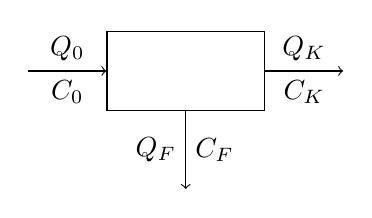
\begin{tikzpicture}
      % Box
      \node[draw, rectangle, minimum width=2cm, minimum height=1cm] (box) at (0, 0) {};
      % Arrows
      \draw[->] (-2, 0) -- (box.west) node[midway, above] {$Q_0$} node[midway, below] {$C_0$};
      \draw[->] (box.east) -- (2, 0) node[midway, above] {$Q_K$} node[midway, below] {$C_K$};
      \draw[->] (box.south) -- (0, -1.5) node[midway, left] {$Q_F$} node[midway, right] {$C_F$};
    \end{tikzpicture}
    \caption{Schematics for solids and fluid balance.}
    \label{fig:balance}
\end{figure}
where:\\
$0$ $\Rightarrow$ inflow (influent),\\
$K$ $\Rightarrow$ cake,\\
$F$ $\Rightarrow$ outflow (filtrate/centrate).
\begin{equation}
    Q_0 = Q_F + Q_K
    \label{eq:liqbalance}
\end{equation}
\begin{equation}
    Q_0C_0 = Q_FC_F + Q_KC_K
    \label{eq:solidsbalance}
\end{equation}
Equation \ref{eq:liqbalance} and Equation \ref{eq:solidsbalance} yields:
\begin{equation}
    Q_K=\frac{Q_0(C_0-C_F)}{(C_K-C_F)}
    \label{eq:balance}
\end{equation}
\% Recovery:
\[
\%R =\frac{\text{mass of dry solids as cake}}{\text{mass of dry feed solids}}*100
\]
\begin{equation}
    \%R =\frac{C_KQ_K}{C_0Q_0}*100
    \label{eq:recovery}
\end{equation}
Substituting Equation \ref{eq:balance} into Equation \ref{eq:recovery}:
\[
\%R =\frac{C_K(C_0-C_F)}{C_0(C_K-C_F)}*100
\]
where:\\
$Q_0$ = feed flow rate,\\
$C_0$ = feed solids concentration,\\
$Q_K$ = filter cake flow,\\
$C_K$ = filter cake solids concentration,\\
$Q_F$ = the filtrate flow,\\
$C_F$ = the solids concentration in the filtrate.
\section*{Chemical Sludges}
\textbf{Alum sludge:}\\
\ce{Al^3+ + PO_4^3- \rightleftarrows AlPO4} $\downarrow$\\
\ce{Al^3+ + 3OH- \rightleftarrows Al(OH)3} $\downarrow$\\
\textbf{Recovery:}\\
\ce{Al(OH)3 + 3H+ \rightarrow Al^3+ + H2O}\\
\textbf{Ferric sludge:}\\
\ce{Fe^3+ + PO_4^3- \rightleftarrows FePO4} $\downarrow$\\
\ce{Fe^3+ + 3OH- \rightleftarrows Fe(OH)3} $\downarrow$\\
\textbf{Lime sludge:}\\
\ce{Ca5(OH)(PO4)3} = calcium hydroxylapatite
\textbf{Quicklime to Slacked/Hydrated lime:}
\ce{CaO + H2O \rightleftarrows Ca(OH)2}
\section*{Sludge Drying and Combustion} \label{Sludge_D_C}
\textbf{H.C.V. or H.H.V. calculations:}
\[
\text{kJ/kg} = 33800 C + 144000 (H - O/8) + 9270 S
\]
\[
\text{BTU/lb} = 14600 C + 62000 (H - O/8) + 4050 S
\]
\[
\text{kcal/kg} = 8080 C + 34500 (H - O/8) + 2240 S
\]
where:\\
C, H, O, S are the weight fractions of corresponding elements.\\
\textbf{Conversions:}
\[
\text{BTU/lb} = \frac{\text{kJ/kg}}{2.326}
\]
\[
\text{kcal/kg} = \frac{\text{kJ/kg}}{4.184}
\]
\[
\text{kcal/kg} = \frac{\text{BTU/lb}}{1.799}
\]
Some empirical formulas can be used to determine the heat value as well:
\[
Q_H = A\left[\frac{100C_V}{100-D}\right] - B\left[\frac{100-D}{100}\right]
\]
or such as,
\[
\text{BTU/lb} = 122C_V - 660
\]
where:\\
$Q_H$ = heat value (BTU/lb),\\
$C_V$ = volatile solids (\%),\\
$D$ = dosage of inorganic chemicals used in dewatering as \% weight of sludge,\\
$A$ = empirical constant (107 for Activated Sludge, 131 for Raw Primary Sludge),\\
$B$ = empirical constant (5 for Activated Sludge, 10 for Raw Primary Sludge).\\
Real heat value calculation:
\[
\text{Real Heat Value} = \text{Heat Value} * f_S * f_V
\]
where:\\
$f_S$ = solid fraction ($\approx$ 0.2--0.25),\\
$f_V$ = volatile fraction ($\approx$ 0.7).
\section*{Regulations of Sludge}
\textbf{\textit{Turkish Regulations}}\\
Su Kirliliği Kontrol Yönetmeliği (Water Pollution Control Regulations)\\
Atıksu Arıtma Tesisleri Teknik Usuller Tebliği (Technical Aspects Bulletin)\\
Atıkların Düzenli Depolanmasına Dair Yönetmelik (Regulation on the Landfilling of Wastes)\\
Atıkların Yakılmasına Dair Yönetmelik (Regulation on the Combustion of Wastes)\\
Evsel ve Kentsel Arıtma Çamurlarının Toprakta Kullanılmasına Dair Yönetmelik (Regulation on the Use of Municipal and Urban Sludges on Land)\\
\textbf{\textit{US Regulations}}\\
Regulated under Federal Regulation in 40 CFR Part 503 Standards for the Use or Disposal of Biosolids.
\end{multicols}
\printbibliography
\end{document}
